\documentclass[12pt, letterpaper]{article}

% font
\usepackage[T1]{fontenc}
\usepackage{hyperref}

% math
\usepackage{mathcomp}
\usepackage{amsmath}

% document formatting
\usepackage{geometry}
\geometry{letterpaper, left=1in, right=1in, top=1in, bottom=1in}
\usepackage{changepage}

% Images
\usepackage{graphicx}
\graphicspath{ {images/} }

% lists
\usepackage{enumitem}

% No indent for entire file
\setlength\parindent{0pt}

% tables
\usepackage{tabularx}
\newcolumntype{S}{@{\stepcounter{Definition}\theDefinition.~} >{}l @{~ : ~}X@{}}
\newcounter{Definition}[subsection]

\usepackage{textcomp}

% graphics
\usepackage{graphicx}
\usepackage{float}
\graphicspath{ {images/} }

% colors
\usepackage{color}
\definecolor{light-gray}{gray}{0.85}

% my own macros!
\usepackage{xspace}
\newcommand{\code}[1]{\colorbox{light-gray}{\texttt{#1}}}
\newcommand{\apr}{\`{a} priori\xspace}

% header / footer
\usepackage{fancyhdr}
\pagestyle{fancy}
\fancyhead{}
\fancyfoot{}
\renewcommand{\headrulewidth}{0.4pt}
\renewcommand{\footrulewidth}{0.4pt}
\fancyhead[LE,RO]{\slshape \leftmark}
\fancyhead[LO,RE]{\slshape \rightmark}
\fancyfoot[LE,RO]{\thepage}

% author tags
\usepackage{authblk}
\renewcommand\Affilfont{\itshape\small}
\renewcommand\Authands{ and }

% multiple columns
\usepackage{multicol}

% code listing
\usepackage{listings}
\lstset{language=FORTRAN} 

\title{FTS Profile Retrieval Pre and Post Processing}

\author[1]{Eric Nussbaumer \thanks{corresponding author: ebaumer@ucar.edu +1 (303) 497-1861}}
\affil[1]{National Center for Atmospheric Research, Boulder, CO, USA}

\date{September 2015}

\begin{document}

\begin{titlepage}

\maketitle
\thispagestyle{empty}
\pagestyle{empty}

\begin{abstract}
  \begin{adjustwidth}{2em}{2em} 
    \large{
      \emph{
This document outlines the creation of the spectral database as well as the profiles for pressure, temperature, and water vapor.
}}
      
  \end{adjustwidth}

\end{abstract}

\end{titlepage}
 
\newpage
%------------------
% Table of contents
%------------------
\tableofcontents
\newpage


\section{Introduction} 
\label{sec:intro}

\section{Pre-Processing}
The spectral database and ZPTW (altitude, pressure, temperature, and water vapor) profiles are necessary pre-processing steps to retrievals. The spectral database holds information pertaining to each of the measurements. A spectral database is unique to each site\\

The majority of information in the spectral database comes from the OPUS file itself; however, we append meteorological data from local weather weather stations.\\

There are several steps in creating the spectral database:\\

\begin{enumerate}
\item Creating the initial spectral database
\item Re-formatting the house log data files
\item Re-formatting the external station weather data
\item Appending the initial spectral database with house an external station weather data
\end{enumerate}

Note that not all sites have house or external station weather data.\\

\begin{tabular}{ l l l }
\textbf{Station} & \textbf{House Data} & \textbf{External Station Data} \\
\hline
MLO   & Yes & Yes (CMDL) \\
TAB   & Yes & No         \\
FL0   & No  & Yes (EOL)  \\
\end{tabular} \\

The necessary python files are located in the \href{https://git.ucar.edu/?p=sfit-processing-environment.git}{sfit-processing-environment} git repository. \\

\subsection{Pulling Data}
\label{sec:PD}
Both the ancillary data as well as the OPUS files need to be downloaded from various sources. The OPUS data is automatically downloaded from MLO and TAB by the program pullRemoteData2.py. This program is set on a cron tab to download data everyday.

The following table shows where the OPUS data is downloaded to.\\

\begin{tabular}{ l l }
\textbf{Data} & \textbf{Local Storage} \\
\hline
MLO   & otserver:/ya4/id/mlo/   \\
TAB   & otserver:/ya4/id/tab/   \\
\end{tabular} \\

The supporting data is pulled with a program using wget. The program is pullAncillaryData.py and is located at: /data/bin/. This program has been setup in cron tab to pull data everyday. The program pullAncillaryData.py gets the following data: NCEP nmc, NCEP I re-analysis, EOL, and CMDL. \\

ERA-Interim data must be manually pulled through the server data-access.ucar.edu.\\

The following table shows the local storage of the ancillary data\\

\begin{tabular}{ l l }
\textbf{Data} & \textbf{Local Storage} \\
\hline
WACCM               & otserver:/data/Campaign/TAB,MLO,FL0/waccm/             \\
NCEP nmc Height     & otserver:/data1/ancillary\_data/NCEP\_NMC/height/      \\
NCEP nmc Temp       & otserver:/data1/ancillary\_data/NCEP\_NMC/temp/        \\
NCEP I Height       & otserver:/data1/ancillary\_data/NCEPdata/NCEP\_hgt/    \\
NCEP I Shum         & otserver:/data1/ancillary\_data/NCEPdata/NCEP\_Shum/   \\
NCEP I Temp         & otserver:/data1/ancillary\_data/NCEPdata/NCEP\_Temp/   \\
NCEP I Trpp         & otserver:/data1/ancillary\_data/NCEPdata/NCEP\_trpp/   \\
ERA-Interim         & otserver:/data1/ancillary\_data/ERAdata/               \\
EOL                 & otserver:/data1/ancillary\_data/fl0/eol/               \\
CMDL Hourly         & otserver:/data1/ancillary\_data/mlo/cmdl/Hourly\_Data/ \\
CMDL Minute         & otserver:/data1/ancillary\_data/mlo/cmdl/Minute\_Data/ \\
\end{tabular} \\

\subsection{Initial Quality Check}
An initial quality check on the spectrum is done using the IDL program ckop.pro. This program allows the user to look through each individual spectra and discard or keep it. Once this is completed the data should be copied over from /ya4/id/(mlo,tab,fl0) to the directory /data1/(mlo,tab,fl0).\\

\begin{tabular}{ l l }
\textbf{Program} & \textbf{Description} \\
\hline
ckop.pro         & IDL program to check OPUS spectra \\
\end{tabular} \\

\section{Spectral Database}
\subsection{Initial Spectral Database}
\label{sec:ISD}
The initial spectral database file is created by running ckopus on the various raw OPUS file. A python program is created to manage the creation of the initial spectral database file (mkSpecDB.py). The program will create a new spectral database file or append an already existing file. Associated with mkSpecDB.py is an input file. The input file allows one to specify the starting and ending date to process, the station, and the various directories and files to use. In addition, one can specify additional ckopus flags to use in the ckopus call. There are logical flags which control the creating of a file which list the folders processed and whether bnr files are created. These files are located under the SpectralDatabase folder of the git repository.\\

\begin{tabular}{ l l }
\textbf{Program} & \textbf{Description} \\
\hline
mkSpecDB.py         & Main program to create initial spectral database \\
specDBInputFile.py  & Input file for mkSpecDB.py program               \\
\end{tabular} \\


\subsection{House Data}
\label{sec:HD}

House data is data that is recorded by the FTS autonomous system, such as outside temperature, pressure, wind direction, etc. The format of this data has changed for each station over time as the instrument gets modified or upgraded. A python program (station\_house\_reader.py) is created to read the various formats and create a standardized file. There is one file for each year. There are no input files for the station\_house\_reader.py program. The time range, station identifier, and directories are specified directly in the program under the main function. An excel spreadsheet describes the various formats for the house log files for MLO and TAB.\\

\begin{tabular}{ l l }
\textbf{Program} & \textbf{Description} \\
\hline
station\_house\_reader.py & Main program to read house data files\\
HouseReaderC.py           & Supporting program with formats of previous house data files \\
HouseDataLog.xlsx         & Excel file with format of house log files\\
\end{tabular} \\

These programs are located in the ExternalData folder of the git repository.


\subsection{External Station Data}
\label{sec:ED}

There are currently two external station data sources used (EOL for FL0, and CMDL for MLO) only the EOL data needs to be pre-processed. The original format of this data is in netcdf files. The program read\_FL0\_EOL\_data.py reads the daily netcdf files and creates a yearly text file. There are no input files for read\_FL0\_EOL\_data.py program. The year of interest and directories of data are specified directly in the program under the main function.  The program pullAncillaryData.py pulls the CMDL and EOL data from each individual ftp site. \\

\begin{tabular}{ l l }
\textbf{Program} & \textbf{Description} \\
\hline
pullAncillaryData.py    & Program to automatically pull EOL and CMDL data\\
read\_FL0\_EOL\_data.py & Main program to read EOL and CMDL data \\
\end{tabular} \\

These programs are located in the ExternalData folder of the git repository.

\subsection{Append Spectral Database File}
\label{sec:ASDF}
The final step is appending the initial spectral database file with the house and external station weather data. A python program was created to accomplish this (appendSpecDB.py). The program appendSpecDB.py reads in the initial spectral database file. It then searches the house and external station files for weather data at the time of observation, plus a certain number of minutes specified by the user. The mean of the data collected is calculated and a new spectral database file is created. If no data is present missing values are used. Associated with appendSpecDB.py is an input file. The input file allows one to specify directories and files, year to process, station, how many minutes to use for averaging, and whether to create a comma separated or pre-specified formatted new spectral database file.\\

\begin{tabular}{ l l }
\textbf{Program} & \textbf{Description} \\
\hline
appendSpecDB.py         & Program to create the append spectral database file\\
appndSpecDBInputFile.py & Input file for appendSpecDB.py \\
\end{tabular} \\

\textit{Note:A warning message will often appear when running this program originating from the python numpy module. This warning is a result of numpy taking the mean of an empty array. This is handled by the main program.}

\section{ZPTW Profiles}
The pressure, temperature, and water vapor profiles can be created from several outside sources. Temperature and pressure profiles are taken from NCEP nmc data; while currently only water profiles are taken from NCEP I and ERA-Interim re-analysis data. Both NCEP and ERA-Interim data are interpolated with WACCM data to reach 120km vertical height. The profiles are daily averages and they reside in the data directories (/data1/tab,mlo,fl0/).\\

The following is a table showing the various reference profiles, their sources, along with the associated file names.\\

\begin{tabular}{ l l l }
\textbf{Profile Type} & \textbf{Source} & \textbf{File Name} \\
\hline
Temperature   & NCEP nmc          & ZPT.nmc.120 \\
Pressure      & NCEP nmc          & ZPT.nmc.120 \\
Water Vapor   & WACCM             & w-120.v1    \\
Water Vapor   & NCEP I            & w-120.v3    \\
Water Vapor   & ERA-Interim       & w-120.v4    \\
Water Vapor   & Retrieved         & w-120.YYYYMMDD.HHMMSS.v99    \\
Water Vapor   & Retrieved Daily   & w-120.v5    \\
\end{tabular} \\


The following table shows the various sources for the data.\\

\begin{tabular}{ l l }
\textbf{Data} & \textbf{Source} \\
\hline
WACCM              & Local (otserver:/data/Campaign/TAB,MLO,FL0/waccm/  \\
NCEP nmc           & ftp://ftp.cpc.ncep.noaa.gov/ndacc/ncep/\\
NCEP I re-analysis & ftp://ftp.cdc.noaa.gov/Datasets/ncep.reanalysis.dailyavgs/          \\
ERA-Interim re-analysis   & /glade/p/rda/data/ds627.0/ei.oper.an.pl/         \\
\end{tabular} \\


\subsection{Pressure \& Temperature Profiles}
\label{sec:PT}
Pressure and temperature profiles in the ZPT.nmc.120 files come from NCEP nmc data. The NCEP nmc data is vertically interpolated with WACCM data to reach 120km. In the event that the NCEP nmc data is not available for a particular day, the WACCM data is substituted.\\

The NCEP nmc data must first be formatted. This is done using the program NCEPnmcFormat.py.\\

After formating the NCEP nmc data one can create the altitude, pressure, and temperature profiles using the program MergPrf.py. This program also creates water profiles from WACCM data (v1).\\

\begin{tabular}{ l l }
\textbf{Program} & \textbf{Description} \\
\hline
NCEPnmcFormat.py & Program to format the NCEP nmc data\\
NCEPinputFile.py & Input file for NCEPnmcFormat.py program \\
MergPrf.py       & Main program to create ZPT and water files from NCEP data\\
mergprfInput.py  & Input file for MergPrf.py program \\
\end{tabular} \\

\subsection{NCEP I \& ERA Interim Water Profiles}
\label{sec:ERAInt}
The ERA-Interim daily profiles are calculated from 6 hourly data. Both the 6 hourly and daily data for profiles are created. The ERA-Interim data is housed locally at NCAR in the CISL Research Data Archive. There is a three month lag between the current date and when the data becomes available. The data is hosted on /glade/ and can be accessed through the data-access.ucar.edu server. The data can be found at: /glade/p/rda/data/ds627.0/ei.oper.an.pl/. The following steps should be used to pre-process the data:\\

\begin{enumerate}
\item Copy over the data from glade
\item Convert GRIB format files to NetCDF files using cnvrtNC.py
\item Create water profiles using ERAwaterPrf.py
\end{enumerate}

The NCEP I re-analysis data are already daily averages. The grid resolution of NCEP I is less than ERA-interim. In addition ERA-Interim assimilates GPS occultation data. It is preferable to use ERA-Interim over NCEP I. The program to create water profiles from NCEP I data is NCEPwaterPrf.py.\\

\begin{tabular}{ l l }
\textbf{Program} & \textbf{Description} \\
\hline
cnvrtNC.py     & Program to convert ERA-Interim GRIB files to NetCDF files\\
ERAwaterPrf.py & Program to extract daily averaged water profiles from ERA-Interim\\
NCEPwaterPrf.py& Program to create daily water profiles from NCEP I\\
\end{tabular} \\


\subsection{Retrieved Water Profiles}
\label{sec:RWP}
For all sites (MLO,TAB, and FL0) water is retrieved when available. This water can be used as a prior for other retrievals. The program retWaterPrf.py creates w-120.YYYYMMDD.HHMMSS.v99 for each retrieval. These files are stored in the data directories (/data1/tab,mlo,fl0/). A daily average of these profiles can be created using the program retWaterPrfDaily.py. These daily averages are also stored in the main data directories (/data1/tab,mlo,fl0/).\\

\begin{tabular}{ l l }
\textbf{Program} & \textbf{Description} \\
\hline
retWaterPrf.py      & Program to create water profiles from water retrieval\\
retWaterPrfDaily.py & Program to create daily average profiles from water retrievals\\
\end{tabular} \\


\subsection{Steps for Pre-Processing}
\label{sec:SCSD}

\begin{itemize}
\item Download OPUS and ancillary data (This is done automatically)
\item Check OPUS spectra
\item Copy spectra from /ya4/id/(mlo,tab,fl0) to /data1/(mlo,tab,fl0)
\item Create initial database
\item Format house data
\item Format external station data
\item Create appended spectral database
\item Create Altitude, Pressure, and Temperature profiles (ZPT.nmc.120)
\item Create water profiles (v1,v2,v3,v4,v5,v99)
\end{itemize}


\section{Processing}
\subsection{Layer0}
The purpose of Layer0 is to run a single retrieval. The program sfit4Layer0.py runs layer 0. This program is called with command line arguments. There is no input file.\\ 

\begin{tabular}{ l l }
\textbf{Program} & \textbf{Description} \\
\hline
sfit4Layer0.py      & Program to run layer 0 using command line arguments\\
\end{tabular} \\

\subsection{Layer1}
The purpose of Layer1 is to batch process multiple or many retrievals. Layer1 requires an input file to specify retrieval options such as date range, input/output directory, etc. In addition, from Layer1 a user can create plots of an individual retrieval. The layer one processing environment serves to do the following:\\

\begin{itemize}
\item Create a directory structure to organize the output data
\item Generate the necessary input files to run SFIT core code
\item Execute the SFIT core code
\item Conduct error analysis on output
\end{itemize}

The following figure shows the input/output flow control for layer 1 processing.

\begin{figure}[H]
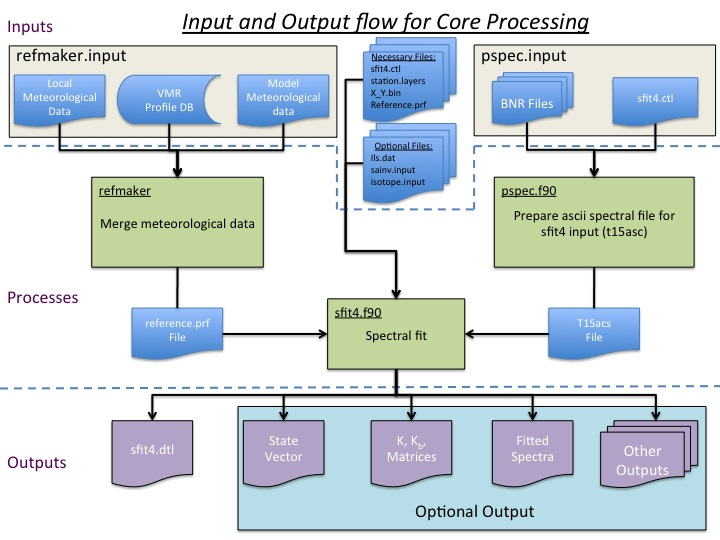
\includegraphics[width=1.0\textwidth]{Slide05}
\caption{A visual representation of the processing flow. }
\label{figure:Layer1Flow}
\end{figure}


\begin{tabular}{ l l }
\textbf{Program} & \textbf{Description} \\
\hline
sfit4Layer1.py      & Program to run layer 1\\
stat\_input.py       & Input file for layer 1\\
mkListFile.py       & Program to create list file from retrieval set (for IDL)\\
\end{tabular} \\

\section{Post-Processing}
\subsection{Plotting}
One can plot individual retrievals or an entire set of retrievals. There are no filtering options for a single retrieval; however, for a set of retrieval there are multiple parameters that one can filter on such as RMS, DOFs, date, etc. The program pltRet.py creates plots for a single retrieval and only requires command line arguments. The program pltSet.py plots an entire set of retrievals and requires an input file (setInput.py).\\

\begin{tabular}{ l l }
\textbf{Program} & \textbf{Description} \\
\hline
pltRet.py      & Program to plot individual retrieval using command line arguments\\
pltSet.py      & Program to plot multiple retrievals using an input file\\
setInput.py    & Input file for pltSet.py\\

\end{tabular} \\

\subsection{HDF Creation}
In order to archive retrievals of NDACC gases one must put the data in a GEOMS complient HDF file (\href{http://avdc.gsfc.nasa.gov/index.php?site=1989220925}{Link}. There is a python routine that converts data to GEOMS HDF4 format. This package of code will also write HDF5 files. In order to run this code there are several software packages that must be install prior to use:

\begin{itemize}
\item The latest HDF4 libraries should be installed on your computer. This library and information on the install can be found at: HDF4
\item If you wish to write HDF5 files, install the python package: h5py (IRWG / GEOMS files are only HDF4.)
\item For writing HDF4 files you need to install the python pyhdf package. We have had to 'tweak' this package for use with GEOMS file format so use the link on the sfit4 wiki page \href{https://wiki.ucar.edu/display/sfit4/Post-Processing}{https://wiki.ucar.edu/display/sfit4/Post-Processing}. Installation instructions for this package are in the INSTALL text file
\item You will also need pythons numpy package
\end{itemize}

The following are a list of files used in the creation of the HDF files:

\begin{itemize}
\item hdfBaseRetDat.py
\item hdfCrtFile.py
\item hdfInitData.py
\item hdfsave.py
\item HDFmain.py
\end{itemize}

The only files that you will need to modify are hdfsave.py, HDFmain.py, and hdfInitData.py. Here is a description of these files:

\begin{itemize}
\item HDFmain.py -- This is an example of how you call the HDFsave object and create an HDF file. From here you define the directory to write the HDF file, whether to write the file using single or double precision, and whether to write an HDF4 or HDF5 file (IRWG / GEOMS are single precision.)
\item hdfsave.py -- This file contains all the global and variable attributes or meta-data. You will need to modify the strings in this file to reflect the specifics of your group, instrument and retrieval process. Remember the formatting of the strings for GEOMS files is VERY specific (e.g. space and capitalization).
\item hdfInitData.py -- This file is the interface between your data and the HDF file. Everyone has data in a specific format so you will need to define a function that takes that data from that format and fills the appropriate class attributes. Currently there are three example interfaces in this file:
\begin{itemize}
\item initIDL -- This interface takes data in from an IDL save file. Note the IDL save file has a specific structure (this idl program is available on request.)
\item initPy  -- This interface can take data using python functions. This interface has not been developed
\item initDummy -- This is a dummy interface which will create dummy (FillValue) data to go into the HDF file.
\end{itemize}
\end{itemize} 

\textcolor{red}{A note on writing data to HDF file:}\\

First, a brief description of the difference between row-major (column is fastest running index) and column-major (row is the fastest running index):\\

Row-major and column-major are methods for storing multidimensional arrays in linear memory. For example, the C language follows row-major convention such that a 2x3 C matrix:\\

\[
C[2,3] =
\begin{pmatrix}
1 & 2 & 3 \\
4 & 5 & 6
\end{pmatrix}
\] 
\\

will be written into linear memory such as: 1,2,3,4,5,6. The rows are written contiguously. The columns are the fastest running index.\\

In Fortran, a 2x3 matrix:

\[
F[2,3] =
\begin{pmatrix}
1 & 2 & 3 \\
4 & 5 & 6
\end{pmatrix}
\] 
\\

will be written into linear memory such as: 1,4,2,5,3,6. The columns are written contiguously. The rows are the fastest running index.\\

How does this translate to higher level dimensions?\\

For column-major convention (Fortran) the fastest running index is furthest left index. For row-major convention (C) the fastest running index is the furthest right index.\\

What does this mean for writing to HDF?\\

HDF uses C storage conventions. It assumes row-major (or the column is the fastest running index). The HDF read and write codes also ensure that the fastest running index is consistent no matter which program (Fortran or C) reads/writes the data. This has implications if you are writing to an HDF file using the Fortran wrapper. From the HDF documentation:

\begin{center}
\textit{"When a Fortran application describes a dataspace to store an array as A(20,100), it specifies the value of the first dimension to be 20 and the second to be 100. Since Fortran stores data by columns, the first-listed dimension with the value 20 is the fastest-changing dimension and the last-listed dimension with the value 100 is the slowest-changing. In order to adhere to the HDF5 storage convention, the HDF5 Fortran wrapper transposes dimensions, so the first dimension becomes the last. The dataspace dimensions stored in the file will be 100,20 instead of 20,100 in order to correctly describe the Fortran data that is stored in 100 columns, each containing 20 elements."}
\end{center}
 

The Fortran wrapper transposes the matrix before it is written to HDF. So the Fortran matrix:\\
\[
F[3,2] =
\begin{pmatrix}
1 & 4 \\
2 & 5 \\
3 & 6
\end{pmatrix}
\] 
\\

Is written to the HDF file as:\\
\[
\begin{matrix}
1 & 2 & 3 \\
4 & 5 & 6 \\
\end{matrix}
\] 
\\

If read using the C wrapper the matrix would look like:\\
\[
\begin{matrix}
1 & 2 & 3 \\
4 & 5 & 6 \\
\end{matrix}
\] 
\\

This makes the values in the fastest running index consistent between Fortran and C. For Fortran the fastest running index are the row (1,2,3) (4,5,6) and for C the fastest running index is the column (1,2,3) (4,5,6). Transposing the matrix before writing and after reading in the Fortran wrapper ensures that the same values are in the fastest running index for Fortran as in C, even though these are different indices in terms of math matrix.\\

The higher-level scripting languages such as Python and IDL use the C set  wrappers, so this is not an issue for them; however, if you are using Matlab to write the data this WILL be an issue. Matlab follows column-major convention (or the rows are the fastest running index). See Matlab documentation.\\

In terms of NDACC GEOMS HDF files this can be an issue for the averaging kernel (AVK) since this matrix is square. The standard for the GEOMS format is that the columns of the AVK  (as described in Rodgers, 2000 pg) should be the fastest running index.\\

So, if you are using column-major (Fortran, Matlab) the dimensions of your AVK when you write to HDF should be:\\

$AVK[ layer\_Index, Kernel_index, Datetime\_index ]$\\

If you are using row-major (C, Python, IDL) the dimensions of your AVK when you write to the HDF should be:\\

$AVK[ Datetime\_index, Kernel_index, layer\_index ]$\\

 
If you have any doubt about how your data is written download either HDF-View or Panalopy or use HDP to view the HDF file you have written. These use C libraries to read the data. When you view the AVK with these programs it should have the following dimensions:  $[datetime, kernel, altitude]$.

\section{Program List}
The following is a list of programs along with a description.

\subsection{Pre-Processing}
\subsection{Spectral Database}
%mkSpecDB.py
\begin{itemize}
\item mkSpecDB.py
\begin{itemize}
\item \textit{Description:} This is the main program to create the spectral database. This program will append a spectral database if one already exists or create a new file. The spectral databases are text files space deliminated. The program looks for .bnr files in the date directories for a given input directory and runs ckopus. The output from ckopus is used to create the initial database. One must have a working version of ckopus.c on their computer in order to create the database. A seperate database is created for each year. This program uses an input file.
\item \textit{Dependencies:} This program requires ckopus.c and an input file (specDBInputFile.py).
\item \textit{Invocation:} mkSpecDB.py -i specDBinputFile.py
\item \textit{Output:} Initial spectral database file. Current location of spectral databases: /data/Campaign/(MLO,TAB)/Spectral\_DB/
\end{itemize}
\end{itemize}

%station_house_reader.py
\begin{itemize}
\item station\_house\_reader.py
\begin{itemize}
\item \textit{Description:} This program reformats the house data log files from MLO and TAB into a single format. The inputs are specified directly in the program file. Even though one can specify a start and stop year, this program should be run for only one year at a time. 
\item \textit{Dependencies:} This program requires HouseReaderC.py which tells the program how to read the various formats of the MLO and TAB house data.
\item \textit{Invocation:} station\_house\_reader.py
\item \textit{Output:} Reformated house log file data. Current directory of reformated house log data: /data/Campaign/(MLO,TAB)/House\_Log\_Files/ 
\end{itemize}
\end{itemize}

%HouseReaderC.py
\begin{itemize}
\item HouseReaderC.py
\begin{itemize}
\item \textit{Description:} This program contains the formats for MLO and TAB house log files.
\item \textit{Dependencies:} None
\item \textit{Invocation:} None
\item \textit{Output:} None
\end{itemize}
\end{itemize}

%HouseDataLog.xlsx
\begin{itemize}
\item HouseDataLog.xlsx
\begin{itemize}
\item \textit{Description:} This program contains a description of the house log files.
\item \textit{Dependencies:} None
\item \textit{Invocation:} None
\item \textit{Output:} None
\end{itemize}
\end{itemize}

%pullAncillaryData.py
\begin{itemize}
\item pullAncillaryData.py
\begin{itemize}
\item \textit{Description:} This program uses the system call "wget" to get NCEP nmc, NCEP re-analysis, EOL, and CMDL data. The output data directories are specified directly in the program. Command line argument allows one to specify the particular date to get data for. This program is set on a cron tab to download data every day. If no date is specified current day is used.
\item \textit{Dependencies:} None
\item \textit{Invocation:} pullAncillaryData.py [-d YYYYMMDD]
\item \textit{Output:} Various directories. See program for output directories.
\end{itemize}
\end{itemize}

%read_FL0_EOL_data.py
\begin{itemize}
\item read\_FL0\_EOL\_data.py
\begin{itemize}
\item \textit{Description:} This program uses the system call "wget" to get NCEP nmc, NCEP re-analysis, EOL, and CMDL data. The output data directories are specified directly in the program. Command line argument allows one to specify the particular date to get data for. This program is set on a cron tab to download data every day. If no date is specified current day is used.
\item \textit{Dependencies:} None
\item \textit{Invocation:} pullAncillaryData.py [-d YYYYMMDD]
\item \textit{Output:} See program for various output directories.
\end{itemize}
\end{itemize}

%appendSpecDB.py
\begin{itemize}
\item appendSpecDB.py
\begin{itemize}
\item \textit{Description:} This program appends already created spectral database files with house and station outside pressure, temperature, and relative humidity values. The inputs are specified with an input file (appndSpecDBInputFile.py). The spectral databases for each year are appended. After the new appended spectral databases are created, the user should concatenate these together into a single database.
\item \textit{Dependencies:} Requires an input file (appndSpecDBInputFile.py)
\item \textit{Invocation:} appndSpecDBInputFile.py -i appndSpecDBInputFile.py
\item \textit{Output:} Appended spectral database file. Current location of spectral databases: /data/Campaign/(MLO,TAB)/Spectral\_DB/
\end{itemize}
\end{itemize}

\subsection{Reference Profiles}
%NCEPnmcFormat.py
\begin{itemize}
\item NCEPnmnFormat.py
\begin{itemize}
\item \textit{Description:} For an individual station this program re-formats the NCEP nmc pressure and temperature data into a single file by year. This program takes an input file (NCEPinputFile.py)
\item \textit{Dependencies:} Requires an input file (NCEPinputFile.py)
\item \textit{Invocation:} NCEPnmnFormat.py -i NCEPinputFile.py
\item \textit{Input:} The input NCEP nmc data is currently located at /data/ancillary\_data/NCEP\_NMC/
\item \textit{Output:} The re-formated NCEP nmc data is currently located at /data/Campaign/(MLO,TAB,FL0)/NCEP\_nmc/
\end{itemize}
\end{itemize}

%MergPrf.py
\begin{itemize}
\item MergPrf.py
\begin{itemize}
\item \textit{Description:} This program creates ZPT files from NCEP nmc data and water files from WACCM data. It requires the use of an input file (mergprfInput.py)
\item \textit{Dependencies:} Requires an input file (mergprfInput.py)
\item \textit{Invocation:} MergPrf.py -i mergprfInput.py
\item \textit{Input:} The input NCEP nmc data is currently located at /data/ancillary\_data/NCEP\_NMC/. The input WACCM data is currently at /data/Campaign/(MLO,TAB,FL0)/waccm/
\item \textit{Output:} The profiles are stored with the bnr data in the daily directories /data1/(mlo,tab,fl0)/
\end{itemize}
\end{itemize}

%cnvrtNC.py
\begin{itemize}
\item cnvrtNC.py
\begin{itemize}
\item \textit{Description:} This program converts the ERA-Interim GRIB files into NetCDF files. This program calls the linux program ncl\_convert2nc to convert the GRIB file to NetCDF. The inputs are directly specified in the program. The NetCDF files are easily readable by python.
\item \textit{Dependencies:} Requires installation of linux program ncl\_convert2nc.
\item \textit{Invocation:} cnvrtNC.py
\item \textit{Input:} The input ERA-Interim (GRIB) data is currently located at /data1/ancillary\_data/ERAdata/
\item \textit{Output:} The output ERA-Interim (NetCDF) data is currently located at /data1/ancillary\_data/ERAdata/
\end{itemize}
\end{itemize}

%ERAwaterPrf.py
\begin{itemize}
\item ERAwaterPrf.py
\begin{itemize}
\item \textit{Description:} This program creates water profiles from the ERA-Interim data. The inputs are directly specified in the program. It interpolates a location and altitude profile to the ERA-Interim grid. It creates daily averages; however, it also stores the 6 hourly PV, Temperature, and Q.
\item \textit{Dependencies:} None
\item \textit{Invocation:} ERAwaterPrf.py
\item \textit{Input:} The input ERA-Interim (NetCDF) data is currently located at /data1/ancillary\_data/ERAdata/
\item \textit{Output:} The output water profiles are stored with the bnr data in the daily directories /data1/(mlo,tab,fl0)
\end{itemize}
\end{itemize}

%NCEPwaterPrf.py
\begin{itemize}
\item NCEPwaterPrf.py
\begin{itemize}
\item \textit{Description:} This program creates water profiles from the NCEP re-analysis data. The inputs are directly specified in the program. It interpolates a location and altitude profile to the NCEP grid. Initial NCEP re-analysis data is already daily averaged.
\item \textit{Dependencies:} None
\item \textit{Invocation:} NCEPwaterPrf.py
\item \textit{Input:} The input NCEP re-analysis (NetCDF) data is currently located at /data1/ancillary\_data/NCEPdata/
\item \textit{Output:} The output water profiles are stored with the bnr data in the daily directories /data1/(mlo,tab,fl0)
\end{itemize}
\end{itemize}

%retWaterPrf.py
\begin{itemize}
\item retWaterPrf.py
\begin{itemize}
\item \textit{Description:} This program creates water a priori profiles retrieved water profiles. The inputs are directly specified in the program. The a priori water profiles are time stamped (date and time) corresponding with measurement time.
\item \textit{Dependencies:} None
\item \textit{Invocation:} retWaterPrf.py
\item \textit{Input:} The input is the location of the retrieved water data.
\item \textit{Output:} The output water profiles are stored with the bnr data in the daily directories /data1/(mlo,tab,fl0)
\end{itemize}
\end{itemize}

%retWaterPrfDaily.py
\begin{itemize}
\item retWaterPrfDaily.py
\begin{itemize}
\item \textit{Description:} This program creates daily averaged water profiles from the a priori water files created from the program retWaterPrf.py. The inputs are specified directly in the program.
\item \textit{Dependencies:} None
\item \textit{Invocation:} retWaterPrfDaily.py
\item \textit{Input:} The input water profiles are located with the bnr data in the daily directories /data1/(mlo,tab,fl0)
\item \textit{Output:} The output water profiles are stored with the bnr data in the daily directories /data1/(mlo,tab,fl0)
\end{itemize}
\end{itemize}

\subsection{Processing}
%sfit4Layer0.py
\begin{itemize}
\item sfit4Layer0.py
\begin{itemize}
\item \textit{Description:} 
\item \textit{Dependencies:} 
\item \textit{Invocation:} 
\item \textit{Input:} 
\item \textit{Output:}
\end{itemize}
\end{itemize}


%sfit4Layer1.py
\begin{itemize}
\item sfit4Layer1.py
\begin{itemize}
\item \textit{Description:} 
\item \textit{Dependencies:} 
\item \textit{Invocation:} 
\item \textit{Input:} 
\item \textit{Output:}
\end{itemize}
\end{itemize}


%mkListFile.py
\begin{itemize}
\item mkListFile.py
\begin{itemize}
\item \textit{Description:} 
\item \textit{Dependencies:} 
\item \textit{Invocation:} 
\item \textit{Input:} 
\item \textit{Output:}
\end{itemize}
\end{itemize}


\subsection{Post-Processing}

\end{document}




